\documentclass[a4paper,11pt]{article}
\usepackage{graphicx}
\usepackage[utf8]{inputenc}
\usepackage{hyperref}
\usepackage{placeins}
\usepackage[newfloat]{minted}
\usepackage{caption}
\usepackage{amssymb}

\newenvironment{code}{\captionsetup{type=listing}}{}
\SetupFloatingEnvironment{listing}{name=Code Overview}


\hypersetup{
    colorlinks=true,
    linkcolor=blue,
    filecolor=black,      
    urlcolor=blue,
    citecolor=black,
}

\begin{document}

\title{
    \textbf{Task 4 Tower of Hanoi}
}
\author{Adrian Jonsson Sjödin}
\date{Spring Term 2023}

\maketitle

\section*{Introduction}
This weeks task was to implement a program able to solve the popular Tower of Hanoi puzzle. To do this we once again use 
recursion to break down the problem into subparts.

\section*{Method}
The strategy to use is described in the task description but I will go through it here again while explaining the code 
seen in code overview \ref{code:hanoi}. 

We start with the base case of when we the number of disks we need to move are zero. For that case we simply return an 
empty list. After this we have the recursive steps which basically works as a recipe and tells how to solve solve the problem.

We start with asking how many disks do you have ({\tt numb\_of\_disks}), which peg are the rings on now ({\tt a}), which peg 
will you use as your temporary peg ({\tt b}), and which peg do you want to move them to {\tt c}? If there are one or more rings
the program will use the recipe to solve the problem step by step. 
\begin{enumerate}
    \item Move all the disks except the last one to the temporary peg \\({\tt hanoi(numb\_of\_disks, a, c, b)}) using the same 
    recipe.
    \item Move the last ring from the original peg to the target peg \\({\tt [\{:move, a, c\}]})
    \item Move the other rings from the temporary peg to the target peg using the same recipe 
    ({\tt hanoi(numb\_of\_disks, b, a, c)})
\end{enumerate}
Each time the recipe, it is a new and smaller version of the problem since one disk has already been moved. Eventually the 
program will run out of disks to move which means the problem is solved. 

We get the instruction of how to move our disks by concatenating together the lists returned by each step of the recipe. 

Worth mentioning is that the tuple {\tt \{:move, a, c\}} means \\{\tt \{:move, source\_peg, target\_peg\}}, they are parameters 
and not fixed values "a" and "c". I realize that the names can be confusing but what is important to remember is that the 
first argument for {\tt hanoi/4} is the number of disks we want to move, the second is the source peg, the third is the temporary 
peg, and the last is the target peg.


\begin{code}
\captionof{listing}{{\tt hanoi/4}}
\label{code:hanoi}
\begin{minted}{elixir}
defmodule Hanoi do
    def hanoi(0, _, _, _) do [] end
    def hanoi(numb_of_disks, a, b, c) do
        hanoi(numb_of_disks-1, a, c, b) ++ 
        [{:move, a, c}] ++ 
        hanoi(numb_of_disks-1, b, a, c)
    end
end
\end{minted}
\end{code}

\section*{Result}
Running the command {\tt Hanoi.hanoi(3, :a, :b, :c)} we get the output seen in code overview \ref{code:hanoi3}, which matches
with the output given in the task instructions. 

\begin{code}
\captionof{listing}{{\tt hanoi(3, :a, :b, :c)}}
\label{code:hanoi3}
\begin{minted}{elixir}
[
  {:move, :a, :c},
  {:move, :a, :b},
  {:move, :c, :b},
  {:move, :a, :c},
  {:move, :b, :a},
  {:move, :b, :c},
  {:move, :a, :c}
]
\end{minted}
\end{code}
In figure \ref{fig:first}-\ref{fig:third} we see that the sequence of moves given in code overview \ref{code:hanoi3} does solve
the puzzle and also the three different sections. Moving all disks except the last one to the temporary peg, then moving the 
last one to the target peg, and lastly moving the other rings from the temporary peg to the target peg. This is exactly like 
we described how the recipe would work in the Method section above.

Lastly to calculate how many moves it takes to solve a tower of size $n$ once can use the formula $2^n -1$. Using this formula 
we get that it would require 1023 moves to move a tower ten disks high from peg A to peg C.

\begin{figure}[ht]
    \begin{minipage}[b]{.45\textwidth}
    \centering
    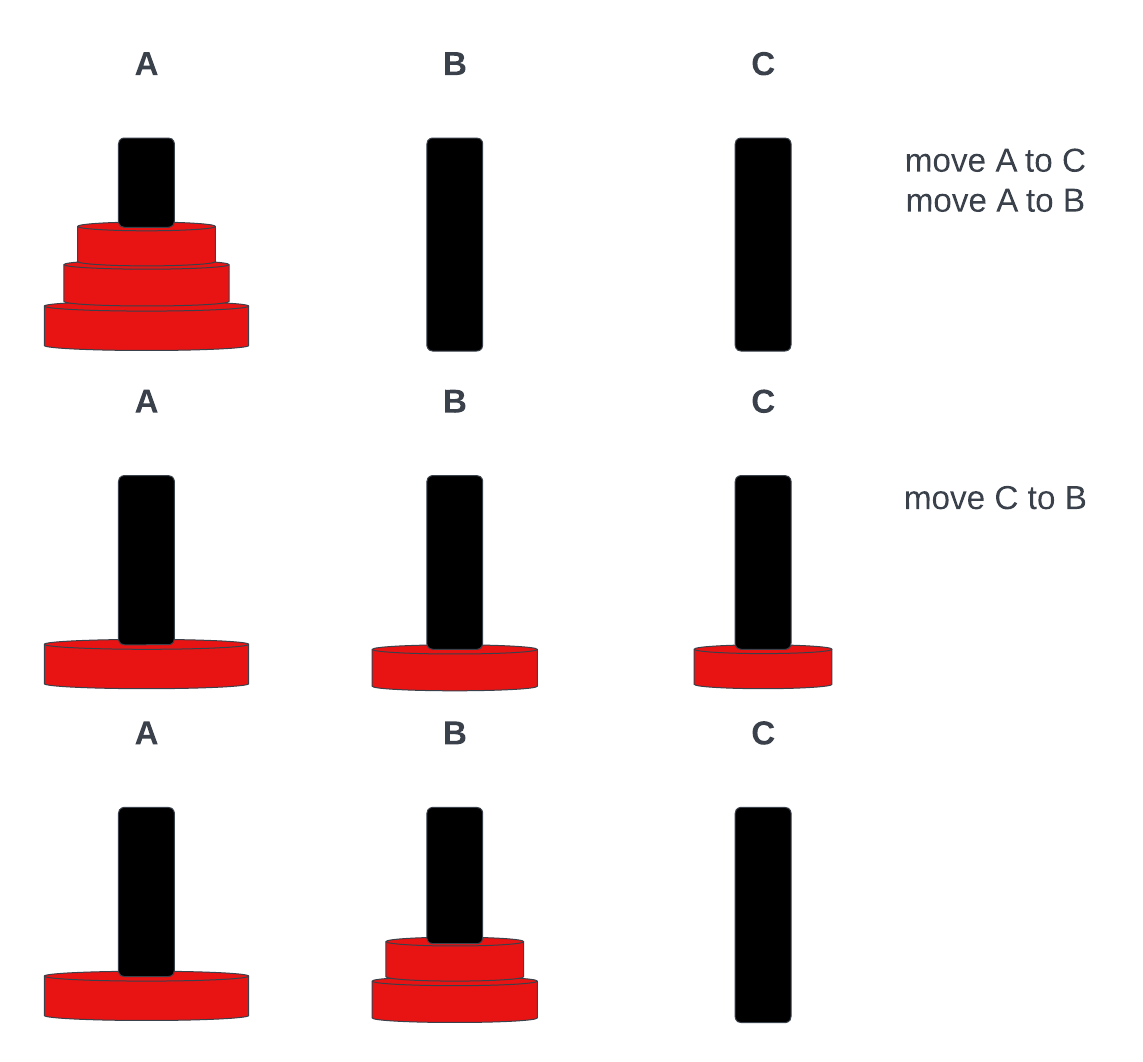
\includegraphics[width=1\textwidth]{hanoi-first-segment.png}
    \caption{First section. Moving \\a tower of two to peg B.}
    \label{fig:first}
    \end{minipage}
    \hfill
    \begin{minipage}[b]{.55\textwidth}
    \centering
    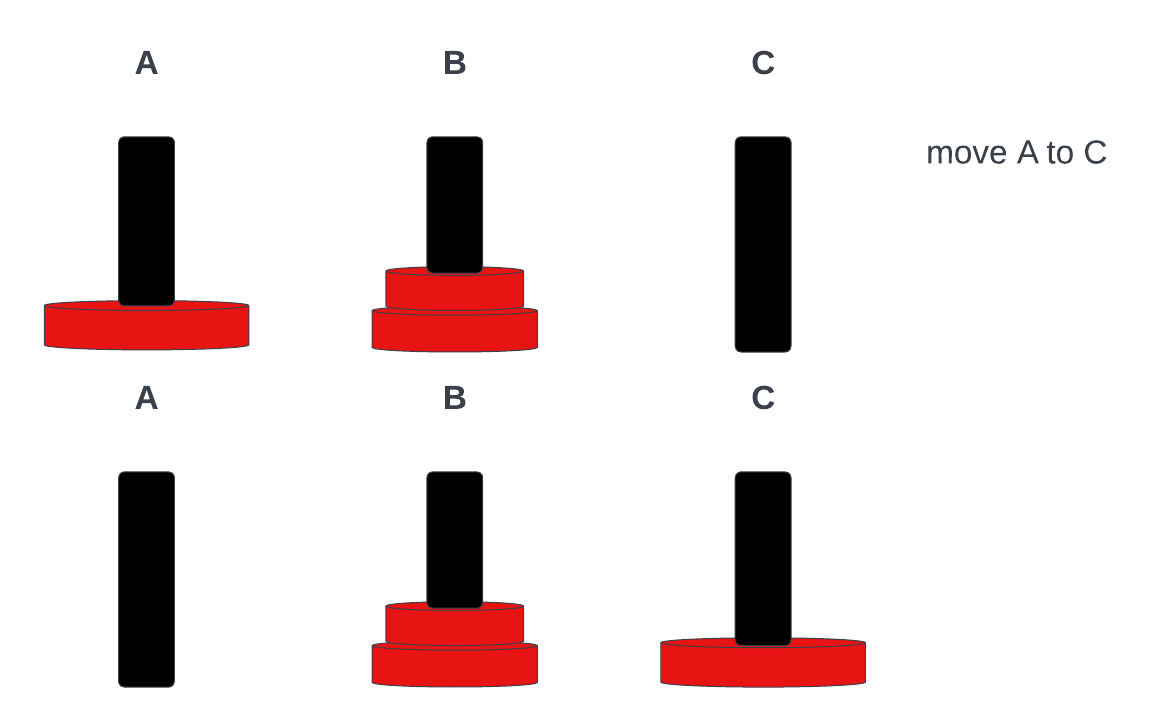
\includegraphics[width=1\textwidth]{hanoi-second-segment.png}
    \caption{Second section. Moving the last disk to peg C.}
    \label{fig:second}
    \end{minipage}
    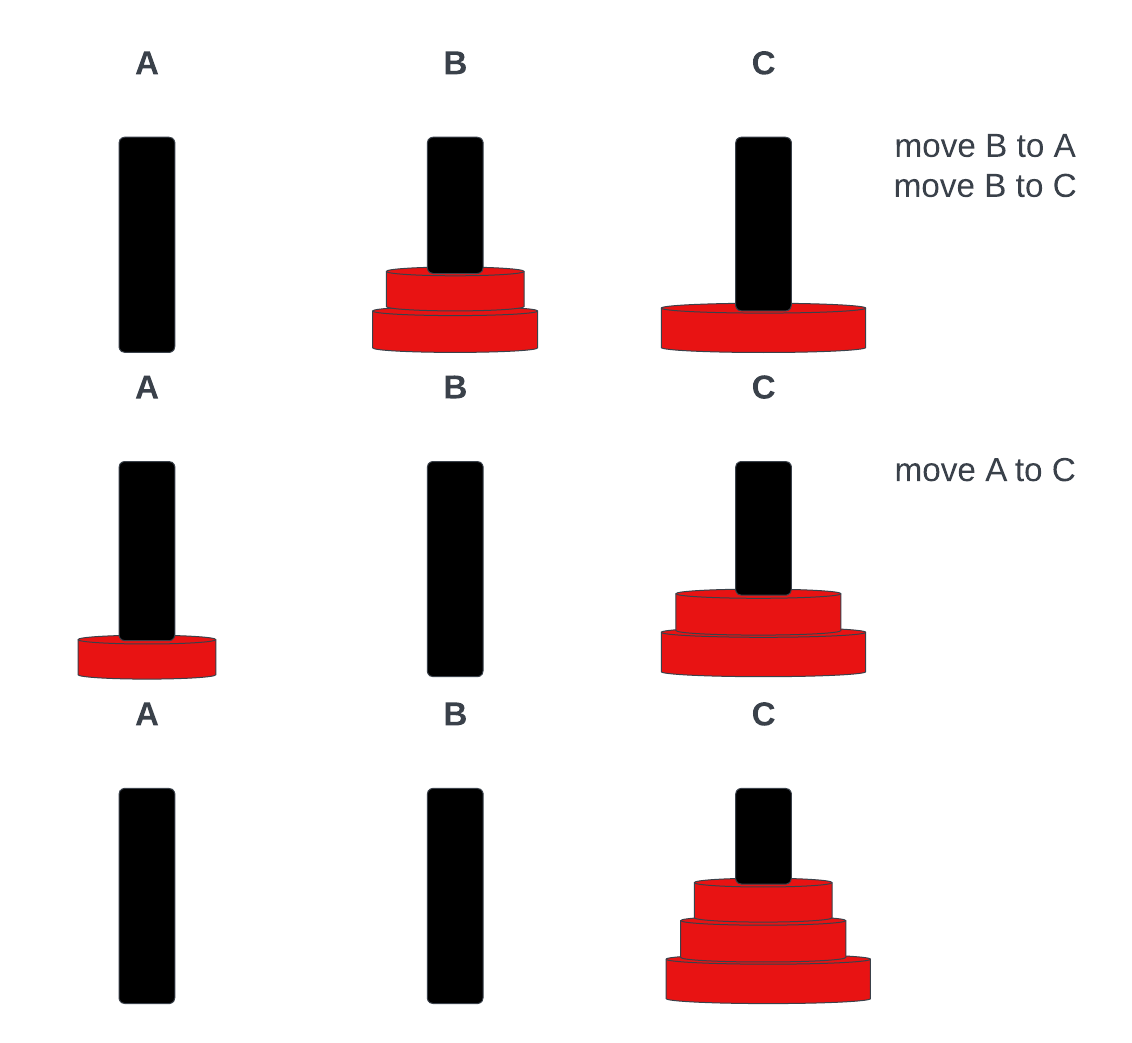
\includegraphics[width=\textwidth]{hanoi-third-segment.png}
    \caption{Third section. Move the tower of two from peg B to peg C.}
    \label{fig:third}
\end{figure}


\FloatBarrier
\section*{Discussion}
There's not really much to discuss when it comes to this task. The way to solve it is described above in the method section
and the code for the {\tt hanoi/4} function is just four lines of code. The hard part was, as in the earlier tasks, the 
recursive part. But having grasped that it was basically just writing down the recipe that we want the program to follow.

You can find the code for this task, and earlier tasks at my
\href{https://github.com/adrian-jonsson-sjoedin/ID1019-Programming-II/tree/main/Task1_Solution}{GitHub}. I have also included 
a function there that implements the formula for calculating the number of moves required to move a tower.




\end{document}
